\documentclass[aspectratio=169]{beamer}
\usepackage[utf8]{inputenc} % codificacao de caracteres
\usepackage[T1]{fontenc}    % codificacao de fontes
\usepackage[english]{babel}  % idioma
\usepackage{graphics,amssymb,amsfonts,amsmath,xfrac}
\usepackage{tikz}
\usepackage{enumerate,hyperref}
\usepackage{palatino}	% Fonte sem serifa
\usepackage{ragged2e}	% Paragrafo justificado
%\usepackage{minted}	% Highlight para codigos de programacao
\usepackage{booktabs} % tabelas
\usepackage{multicol}
\usepackage{multirow}

%\usepackage[table]{xcolor}


% Veja mais temas e cores em http://www.hartwork.org/beamer-theme-matrix/
\usetheme{Montpellier}         % tema
\usecolortheme{orchid}      % cores
\usefonttheme[onlymath]{serif} % fonte modo matematico
% Colocando numero de paginas no slide
\setbeamertemplate{footline}[frame number]



\DeclareGraphicsExtensions{.pdf,.JPG,.png} % compilamos apenas com pdflatex
%\graphicspath{{./figuras/}} % caminho onde as figuras estarao disponiveis


\graphicspath{{figuras/}}

% ---------------------------------------------------------------------------- %
% T�tulo                                                                       %
% ---------------------------------------------------------------------------- %

\title[\sc{Teoria de Circuitos Eletrônicos 1}]{\LARGE Aula 11 - The Complete Response of Circuits
with Two Energy Storage Elements}
\author[Prof. Marcelino Andrade]{Prof. Marcelino Andrade}
\institute{Faculdade UnB Gama} % opcional
\date{\today}

\begin{document}
\justifying % Paragrafo justificado
\pagebreak

\begin{frame}
  \titlepage
\end{frame}


% ----------------- NOVO SLIDE --------------------------------
\begin{frame}{Contents}

\tableofcontents
%\begin{center}	
     		Introduction to Electric Circuits by James A. Svoboda, Richard C. Dorf, 9th Edition 
  %   		Fundamentals of Electric Circuits by Alexander and Sadiku, 4th Edition	
%\end{center}	
\end{frame}

% ----------------- NOVA SECÇÂO -----------------------------
\section{Introduction (9.1)}
% ----------------- NOVO SLIDE --------------------------------
\begin{frame}[fragile]
	\frametitle{Introduction}
		\begin{tabular}{cc}
			\begin{columns}
				\begin{column}{1\textwidth}  %%<--- here
					In this chapter, we consider second-order circuits. To find the response of the second-order circuit, we:	
		
\footnotesize		\begin{itemize}
						\item[$\clubsuit$]{Represent the circuit by a second-order differential equation.\newline}
						\item[$\clubsuit$]{Find the general solution of the homogeneous differential equation.\newline}
						\item[$\clubsuit$]{Find a particular solution of the differential equation.\newline}	
						\item[$\clubsuit$]{Represent the response of the second-order circuit as $x(t)=x_n(t)+ x_f(t)$.\newline}	
						\item[$\clubsuit$]{Use the initial conditions to evaluate the unknown constants.\newline}	
					\end{itemize}
					
				\end{column}
			\end{columns}
		
	\end{tabular}
\end{frame}

% ----------------- NOVA SECÇÂO -----------------------------
\section{Differential Equation for Circuits with Two Energy Storage Elements (9.2)}
% ----------------- NOVO SLIDE --------------------------------
\begin{frame}[fragile]
	\frametitle{The Direct Method}
		\begin{tabular}{cc}
		\begin{columns}
		\begin{column}{1\textwidth}  %%<--- here
\small					\textbf{The Direct Method for Obtaining the Second-Order Differential Equation
of a Circuit} \newline
%\end{center}			
				\end{column}
			\end{columns}\\
					\begin{columns}
		\begin{column}{1\textwidth}  %%<--- here
\small					\textbf{Step 1:} Identify the first and second variables, $x_1$ and $x_2$. These variables are capacitor voltages and/or inductor
currents.
%\end{center}			
				\end{column}
			\end{columns}\\
\begin{columns}
	\begin{column}{.5\textwidth}  %%<--- here
	\center			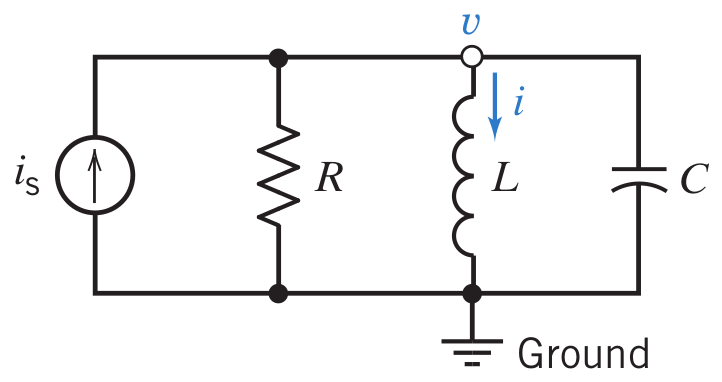
\includegraphics[height=2.5cm]{figure1.png}\\
				\end{column}
	\begin{column}{.5\textwidth}  %%<--- here\
	\center			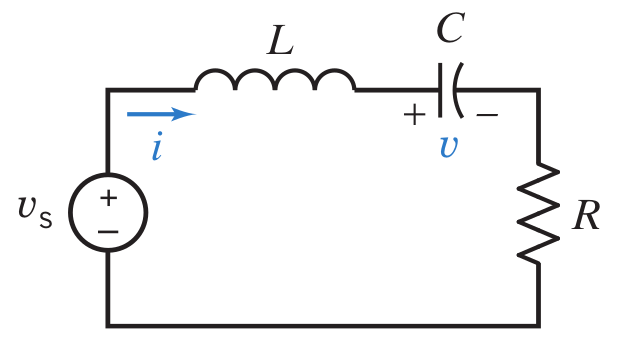
\includegraphics[height=2.5cm]{figure2.png}\\
				\end{column}				
		\end{columns}\\
\begin{columns}
	\begin{column}{.5\textwidth}  %%<--- here
\small \center			A parallel RLC circuit.
				\end{column}
	\begin{column}{.5\textwidth}  %%<--- here
\small \center		A series RLC circuit.
				\end{column}		
		\end{columns}\\		
	\end{tabular}		
\end{frame}
% ----------------- NOVO SLIDE --------------------------------

\begin{frame}[fragile]
	\frametitle{The Direct Method}
		\begin{tabular}{cc}

		\begin{columns}
		\begin{column}{1\textwidth}  %%<--- here
\small		\textbf{Step 2:} Write one first-order differential equation, obtaining $\frac{dx_1}{dt}=f(x_1,x_2)$.
%\end{center}			
		\end{column}
		\end{columns}\\
	\begin{columns}
	\begin{column}{.5\textwidth}  %%<--- here
\center		$-i_s+\frac{v}{R}+i+C\frac{dv}{dt}=0$\\
				\end{column}
	\begin{column}{.5\textwidth}  %%<--- here\
\center		$-v_s+L\frac{di}{dt}+v+Ri=0$\\
				\end{column}				
	\end{columns}\\
		\begin{columns}
		\begin{column}{1\textwidth}  %%<--- here
\small	\newline	\textbf{Step 3:} Obtain an additional first-order differential equation in terms of the second variable so that 
$\frac{dx_2}{dt}=Kx_1$ or $x_1=\frac{1}{K}\frac{dx_2}{dt}$.
%\end{center}			
		\end{column}
		\end{columns}\\
	\begin{columns}
	\begin{column}{.5\textwidth}  %%<--- here
\center				$v=L \frac{di}{dt}$\\
				\end{column}
	\begin{column}{.5\textwidth}  %%<--- here\
\center				$i=C \frac{dv}{dt}$\\
				\end{column}				
	\end{columns}\\	
		\begin{columns}
		\begin{column}{1\textwidth}  %%<--- here
\small		\textbf{Step 4:} Substitute the equation of step 3 into the equation of step 2, thus obtaining a second-order differential
equation in terms of $x_2$.
%\end{center}			
		\end{column}
		\end{columns}\\
	\begin{columns}
	\begin{column}{.5\textwidth}  %%<--- here
\center		$\frac{L}{R}\frac{di}{dt}+i+CL\frac{d^2i}{dt^2}=i_s$\\
		$\frac{d^2i}{dt^2}+\frac{1}{RC}\frac{di}{dt}+\frac{1}{CL}i=\frac{1}{CL}i_s$\\
		
				\end{column}
	\begin{column}{.5\textwidth}  %%<--- here\
\center		$LC\frac{d^2v}{dt^2}+v+RC\frac{dv}{dt}=v_s$\\
		$\frac{d^2v}{dt^2}+\frac{R}{L}\frac{dv}{dt}+\frac{1}{RC}v=\frac{1}{LC}v_s$\\
				\end{column}				
	\end{columns}\\		
	
	\end{tabular}		
\end{frame}

% ----------------- NOVO SLIDE --------------------------------
\begin{frame}[fragile]
	\frametitle{The Operator Method}
		\begin{tabular}{cc}
		\begin{columns}
		\begin{column}{1\textwidth}  %%<--- here
\small					\textbf{Operator Method for Obtaining the Second-Order Differential Equation
of a Circuit} \newline
%\end{center}			
				\end{column}
			\end{columns}\\
\begin{columns}
	\begin{column}{.5\textwidth}  %%<--- here
	\small					\textbf{Step 1:} Identify the variable $x_1$ for which the solution is desired.
	\center			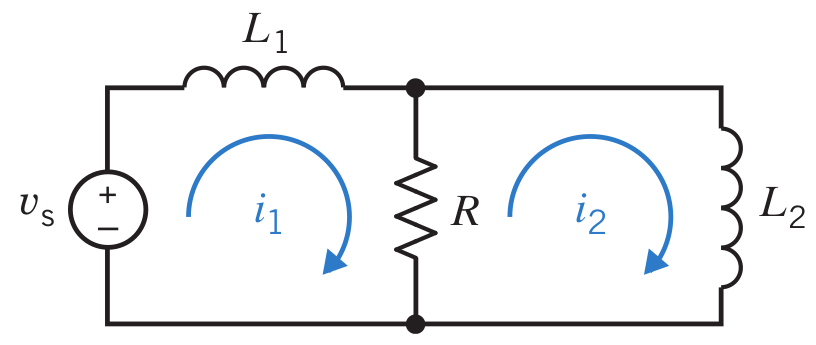
\includegraphics[height=2.5cm]{figure3.png}\\
				\end{column}
	\begin{column}{.5\textwidth}  %%<--- here\
	\small			\textbf{Step 2:} Write one differential equation in terms of the desired variable $x_1$ and a second variable, $x_2$.\\
	\center		$L_1\frac{di_1}{dt}+Ri_1-Ri_2=v_s$\\
	\flushleft \small			\textbf{Step 3:} Obtain an additional equation in terms of the second variable and the first variable.\\
	\center		$L_2\frac{di_2}{dt}+Ri_2-Ri_1=0$\\
				\end{column}				
		\end{columns}\\
\begin{columns}
	\begin{column}{.5\textwidth}  %%<--- here
\small \center			$i_2?$
				\end{column}
	\begin{column}{.5\textwidth}  %%<--- here
\small \center		.
				\end{column}		
		\end{columns}\\		
	\end{tabular}		
\end{frame}

% ----------------- NOVO SLIDE --------------------------------
\begin{frame}[fragile]
	\frametitle{The Operator Method}
		\begin{tabular}{cc}

\begin{columns}
	\begin{column}{.5\textwidth}  %%<--- here
	\small	\textbf{Step 4:} Use the operator $s=\frac{d}{dt}$ and $\frac{1}{s}=\int dt $ to obtain two algebraic equations in terms of s and the two
variables $x_1$ and $x_2$.\\
	\center		$L_1Si_1+Ri_1-Ri_2=v_s$\\
		$L_2Si_2+Ri_2-Ri_1=0$\\

				\end{column}
	\begin{column}{.5\textwidth}  %%<--- here\
	\small	\textbf{Step 6:} Rearrange the equation of step 5 so that $Q(s)x_1=P(s)$. \\
	\center		$[L_1L_2S^2+(L_1R+L_2R)S]i_2=Rv_s$ \\
				\end{column}				
		\end{columns}\\
\begin{columns}
	\begin{column}{.5\textwidth}  %%<--- here

 \small	 \textbf{Step 5:} Using Cramer’s rule, solve for the desired variable so that $x_1= \frac{P(s)}{Q(s)}$, where $P(s)$
and $Q(s)$ are polynomials in $s$.\\
	\center		$i_2=\frac{Rv_s}{L_1L_2S^2+(L_1R+L_2R)S}$ \\
				\end{column}
	\begin{column}{.5\textwidth}  %%<--- here\
 \small	\textbf{Step 7:} Convert the operators back to derivatives for the equation of step 6 to obtain the second-order differential
equation.\\
	\center		$L_1L_2\frac{d^2i_2}{dt}+(L_1R+L_2R)\frac{di_2}{dt}=Rv_s$ \\
				\end{column}				
		\end{columns}\\
	\end{tabular}		
\end{frame}



% ----------------- NOVO SLIDE --------------------------------
\begin{frame}[fragile]
	\frametitle{Differential Equation}
\begin{tabular}{ll}
	\begin{columns}
		\begin{column}{1\textwidth}  %%<--- here
		\textbf{EXAMPLE 9.2-2} - Find the differential equation for the voltage $v$ for the circuit of Figure Below.\\
		\begin{center}
    			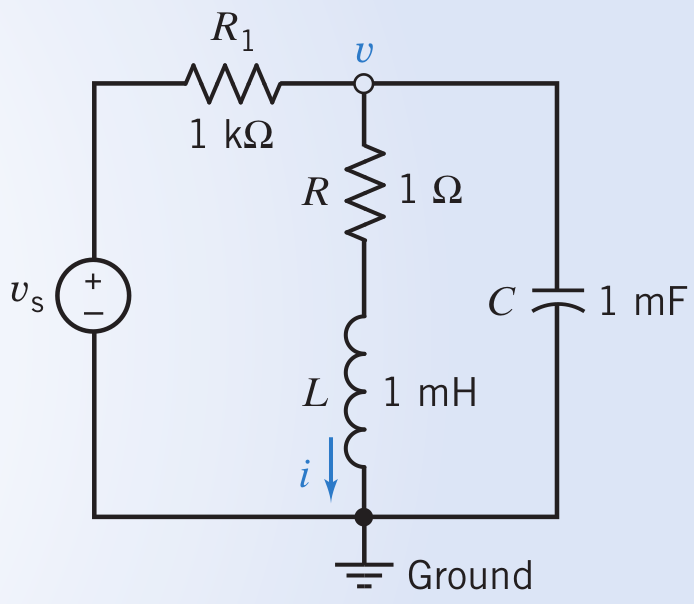
\includegraphics[height=3cm]{figure4.png}	
		\end{center}	
		\scalebox{0.8}{Answer: $\frac{d^2v}{dt^2}+1001\frac{dv}{dt}+1001x10^3v=\frac{dv_s}{dt}+1000v_s$}
		\end{column}
	\end{columns}
\end{tabular}
\end{frame}
% ----------------- NOVO SLIDE --------------------------------
\begin{frame}[fragile]
	\frametitle{Differential Equation}
\begin{tabular}{ll}
	\begin{columns}
		\begin{column}{1\textwidth}  %%<--- here
		\textbf{EXERCISE 9.2-1} - Find the second-order differential equation for the circuit
shown in Figure Below in terms of $i$, using the direct method.\\
		\begin{center}
    			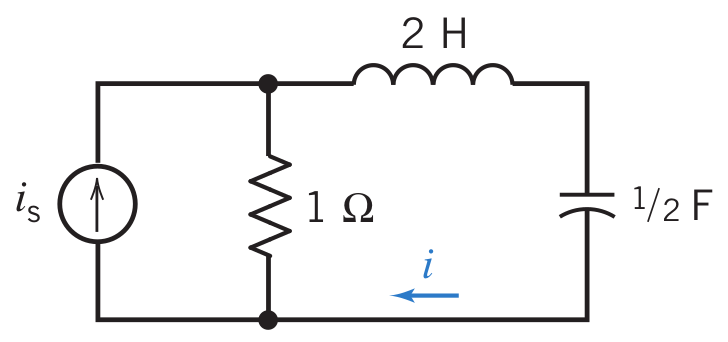
\includegraphics[height=3cm]{figure5.png}	
		\end{center}	
		\scalebox{0.8}{Answer: $\frac{d^2i}{dt^2}+\frac{1}{2}\frac{di}{dt}+i=\frac{1}{2}\frac{di_s}{dt}$}
		\end{column}
	\end{columns}
\end{tabular}
\end{frame}
% ----------------- NOVO SLIDE --------------------------------
\begin{frame}[fragile]
	\frametitle{Differential Equation}
\begin{tabular}{ll}
	\begin{columns}
		\begin{column}{1\textwidth}  %%<--- here
		\textbf{EXERCISE 9.2-2} - Find the second-order differential equation for the circuit
shown in Figure Below in terms of $v$ using the operator method.\\
		\begin{center}
    			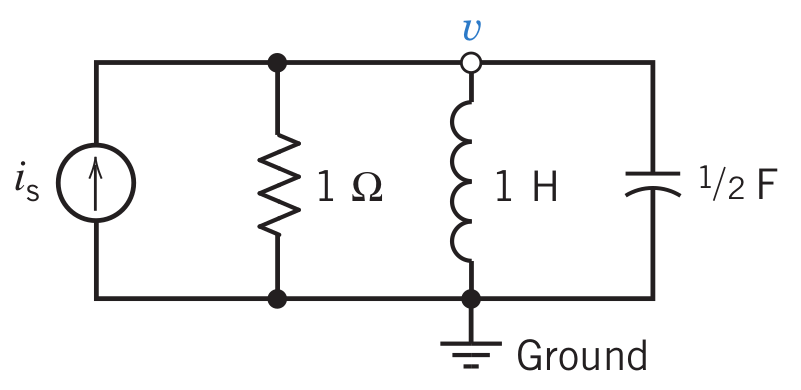
\includegraphics[height=3cm]{figure6.png}	
		\end{center}	
		\scalebox{0.8}{Answer: $\frac{d^2v}{dt^2}+{2}\frac{dv}{dt}+2v={2}\frac{di_s}{dt}$}
		\end{column}
	\end{columns}
\end{tabular}
\end{frame}
% ----------------- NOVA SECÇÂO -----------------------------

\section{Solution of the Second-Order Differential Equation—The Natural Response (9.3)}
% ----------------- NOVO SLIDE --------------------------------
\begin{frame}[fragile]
	\frametitle{The Natural Response}

		\begin{tabular}{cc}
			\begin{columns}
\small				\begin{column}{1\textwidth}  %%<--- here
					In the preceding section, we found that a circuit with two irreducible energy storage elements can be
represented by a second-order differential equation of the form. 
\begin{center}
$a_2\frac{d^2x(t)}{dt^2}+a_1\frac{dx(t)}{dt}+a_0x(t)=f(t)$

\end{center}
where the constants $a_2$ , $a_1$ , $a_0$ are known and the forcing function $f(t)$ is specified.
The complete response $x(t)$ is given by
\begin{center}
$x(t)=x_n(t)+x_f(t)$
\end{center}
where $x_n(t)$ is the natural response and $x_f(t)$ is a forced response. \newline \newline The natural response satisfies the unforced
differential equation when $f(t)=0$. The forced response $x_f(t)$ satisfies the differential equation with the
forcing function present.
		
				\end{column}
			\end{columns}\\	
	\end{tabular}	
\end{frame}
% ----------------- NOVO SLIDE --------------------------------
\begin{frame}[fragile]
	\frametitle{The Natural Response}

		\begin{tabular}{cc}
			\begin{columns}
\small				\begin{column}{1\textwidth}  %%<--- here
					The natural response of a circuit $x_n$ will satisfy the equation 
\begin{center}
$a_2\frac{d^2x(t)}{dt^2}+a_1\frac{dx(t)}{dt}+a_0x(t)=0$

\end{center}
Because $x_n$ and its derivatives must satisfy the equation, we postulate the exponential solution
\begin{center}
$x_n(t)=Ae^{st}$
\end{center}
where $A$ and $s$ are to be determined. Thus, we have
		\footnotesize	\begin{center}  
		
				$a_2As^2e^{st}+a_1Ase^{st}+a_0Ae^{st}=0$ \\   
				$(a_2s^2+a_1s+a_0)Ae^{st}=0 $\\
				$a_2s^2+a_1s+a_0=0$
				\end{center}
				
				\end{column}
			\end{columns}\\	
	\end{tabular}	
\end{frame}

% ----------------- NOVO SLIDE --------------------------------

% ----------------- NOVO SLIDE --------------------------------
\begin{frame}[fragile]
	\frametitle{The Natural Response}

		\begin{tabular}{cc}
			\begin{columns}
\small				\begin{column}{1\textwidth}  %%<--- here
The \textbf{characteristic equation} is derived from the governing differential equation for a circuit
by setting all independent sources to zero value and assuming an exponential solution.
\begin{center}
$a_2s^2+a_1s+a_0=0$

\end{center}
The solution of the characteristic equation has two roots, $s_1$ and $s_2$, where
\begin{center}
$s_1=\frac{-a_1+\sqrt{a_1^2-4a_2a_0}}{2a_2} \ and \ s_2=\frac{-a_1-\sqrt{a_1^2-4a_2a_0}}{2a_2}$
\end{center}
When there are two distinct roots, the natural response is of the form
		\footnotesize	\begin{center}  
		
				$x_n=A_1e^{s_1t}+A_2e^{s_2t}$ \\   
				\end{center}
Where $A_1$ and $A_2$ are unknown constants that will be evaluated later. The \textbf{roots} of the characteristic equation contain all the information necessary for determining
the character of the natural response.			
				\end{column}
			\end{columns}\\	
	\end{tabular}	
\end{frame}
% ----------------- NOVO SLIDE --------------------------------
\begin{frame}[fragile]
	\frametitle{The Natural Response}
\begin{tabular}{ll}
	\begin{columns}
		\begin{column}{1\textwidth}  %%<--- here
		\textbf{EXAMPLE 9.3-1} - Find the natural response of the circuit current $i_2$ shown in
Figure Below. Use operators to formulate the differential equation and obtain the response in terms of two arbitrary constants.\\
		\begin{center}
    			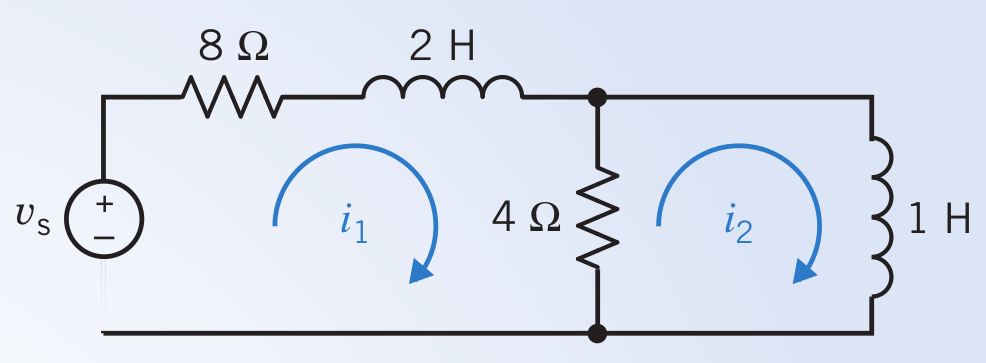
\includegraphics[height=2.7cm]{figure7.png}	
		\end{center}	
		\scalebox{0.8}{Answer: $x_n(t)=A_1e^{-2t}+A_2e^{-8t}$ }
		\end{column}
	\end{columns}
\end{tabular}
\end{frame}
% ----------------- NOVO SLIDE --------------------------------
\begin{frame}[fragile]
	\frametitle{The Natural Response}
\begin{tabular}{ll}
	\begin{columns}
		\begin{column}{1\textwidth}  %%<--- here
		\textbf{EXERCISE 9.3-1} - Find the characteristic equation and the natural frequencies for the circuit
shown in Figure Below.\\
		\begin{center}
    			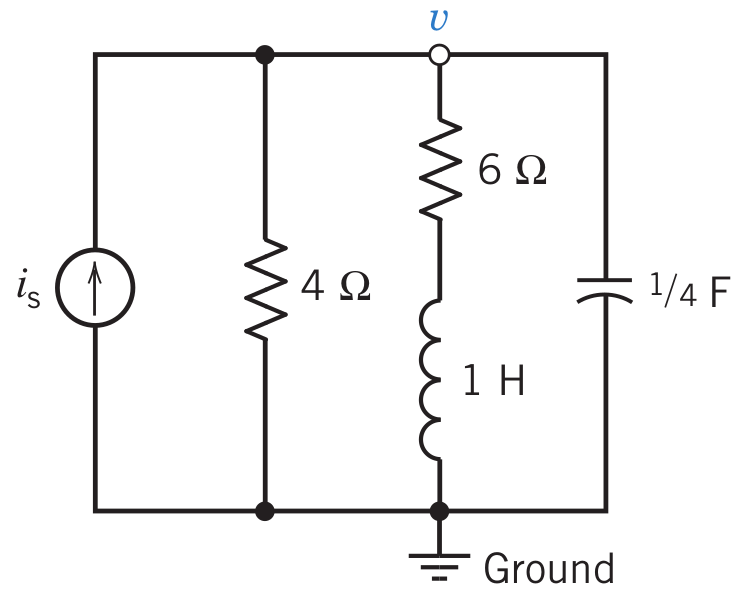
\includegraphics[height=3.3cm]{figure8.png}	
		\end{center}	
		\scalebox{0.8}{Answer: $s^2+7s+10=0$ }
		\end{column}
	\end{columns}
\end{tabular}
\end{frame}
% ----------------- NOVA SECÇÂO -----------------------------
\section{Natural Response of the Unforced Parallel RLC Circuit (9.4)}
% ----------------- NOVO SLIDE --------------------------------
\begin{frame}[fragile]
	\frametitle{Parallel RLC Circuit}
\begin{tabular}{ll}
	\begin{columns}
		\begin{column}{.5\textwidth}  %%<--- here
		In this section, we consider the (unforced) natural response of the parallel RLC circuit shown
in Figure Below\\
		\begin{center}
    			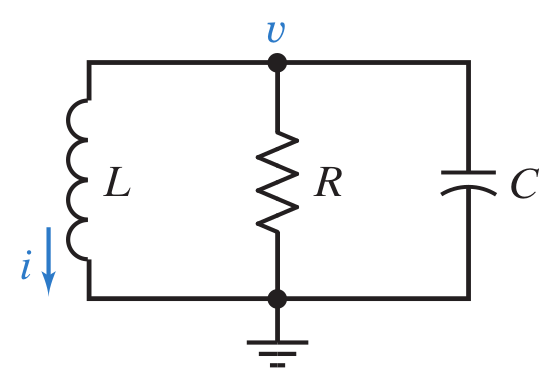
\includegraphics[height=3.5cm]{figure9.png}	
		\end{center}	


		\end{column}

		\begin{column}{.5\textwidth}  %%<--- here
	
The circuit shown does not contain any independent sources, so the input $f(t)$ is
zero. \newline \newline The differential equation is called a homogeneous.
	\begin{center}  
		
				$\frac{d^2x(t)}{dt^2}+2 \alpha \frac{dx(t)}{dt}+\omega_0^2x(t)=0$\\   
				\end{center}

The coefficients of this differential equation have names: $\alpha$ is called the damping coefficient, and
$\omega_0$ is called the resonant frequency.

		\end{column}		
	\end{columns}
\end{tabular}	
\end{frame}
% ----------------- NOVO SLIDE --------------------------------
\begin{frame}[fragile]
	\frametitle{Parallel RLC Circuit}
\begin{tabular}{ll}
	\begin{columns}
		\begin{column}{.6\textwidth}  %%<--- here
The differential equation:
		\begin{center}
		$\frac{v}{R}+\frac{1}{L} \int_{0}^{t} v d \tau + i(0) + C\frac{dv}{dt}=0$ \newline \\
		  $C\frac{d^2v}{dt^2} + \frac{1}{R}\frac{dv}{dt}+\frac{1}{L}v=0$  \newline  \\ 
		$\frac{d^2v}{dt^2} + \frac{1}{RC}\frac{dv}{dt}+\frac{1}{LC}v=0$ \newline  \\
		$s^2v + \frac{1}{RC}sv+\frac{1}{LC}v=0$\newline  \\
	
		 \end{center}		
		 Characteristic  Equation: $s^2 + \frac{1}{RC}s+\frac{1}{LC}=0$

		 
		 \end{column}

		\begin{column}{.5\textwidth}  %%<--- here
We can see \newline
		\begin{center}
		$\frac{d^2x(t)}{dt^2}+2 \alpha \frac{dx(t)}{dt}+\omega_0^2x(t)=0$ \newline \\
		$\frac{d^2v(t)}{dt^2} + \frac{1}{RC}\frac{dv(t)}{dt}+\frac{1}{LC}v(t)=0$ \newline  \\ 	
		 \end{center}		
Thus

		\begin{center}
		$\alpha = \frac{1}{2RC}$ \ and \ 
		  $\omega_o^2=\frac{1}{LC}$    \\ 	
		 \end{center}	



		\end{column}		
	\end{columns}
\end{tabular}	
\end{frame}
% ----------------- NOVO SLIDE --------------------------------
\begin{frame}[fragile]
	\frametitle{Parallel RLC Circuit}
\begin{tabular}{ll}
\small	\begin{columns}
		\begin{column}{.5\textwidth}  %%<--- here
The Characteristic  Equation:
		\begin{center}
		$s^2 + \frac{1}{RC}s+\frac{1}{LC}=0$
		 \end{center}		
The two roots of the characteristic equation are
		\begin{center}
\footnotesize $s_1=-\frac{1}{2RC}+\sqrt{(\frac{1}{2RC})^2-\frac{1}{LC}}$ 
\footnotesize $s_2=-\frac{1}{2RC}-\sqrt{(\frac{1}{2RC})^2-\frac{1}{LC}}$ \\				
		 \end{center}	
The solution to the second-order differential for t > 0 is
		\begin{center}
		$v_n=A_1e^{s_1t}+A_2e^{s_2t}$ \newline \\ 	
		 \end{center}
		 \end{column}

\small		\begin{column}{.5\textwidth}  %%<--- here
	
The roots of the characteristic equation may be rewritten as
		\begin{center}
\footnotesize		$s_1=-\alpha+\sqrt{\alpha^2-\omega_0^2}$ \ and \ $s_2=-\alpha-\sqrt{\alpha^2-\omega_0^2}$    \\ 	
		 \end{center}	
The damped resonant frequency, $\omega_d$, is defined to be
		\begin{center}
		$\omega_d=\sqrt{\omega_0^2-\alpha^2}$    \\ 	
		 \end{center}	
When $\omega_0>\alpha$, the roots of the characteristic equation are complex and can be expressed as
\footnotesize		\begin{center}
		$s_1=-\alpha+j\omega_d$ \ and \ $s_1=-\alpha-j\omega_d$    \\ 	
		 \end{center}	

		\end{column}		
	\end{columns}
\end{tabular}	
\end{frame}
% ----------------- NOVO SLIDE --------------------------------
\begin{frame}[fragile]
	\frametitle{Parallel RLC Circuit}
		\begin{tabular}{cc}
			\begin{columns}
				\begin{column}{1.1\textwidth}  %%<--- here
The roots of the characteristic equation assume three possible conditions: 


		\begin{enumerate}
						\item{Two real and distinct roots when $\alpha^2>\omega_0^2$.}
						\begin{itemize}
						 \item When the two roots are real and distinct, the circuit is said to be \textbf{\textit{overdamped}}. \newline.
						\end{itemize}						
						\item{Two real equal roots when $\alpha^2=\omega_0^2$.}
						\begin{itemize}
						 \item When the roots are both real and equal, the circuit is \textbf{\textit{critically damped}}. \newline.
						\end{itemize}
						\item{Two complex roots when $\alpha^2<\omega_0^2$.}
						\begin{itemize}
						 \item When the two roots are complex conjugates, the circuit is said to be \textbf{\textit{underdamped}}. \newline.
						\end{itemize}
					\end{enumerate}
					
				\end{column}
			\end{columns}\\
$s_{1,2}=-\alpha \pm \sqrt{\alpha^2-\omega_0^2}$, \ $\omega_d=\sqrt{\omega_0^2-\alpha^2}$ \ and \ $s_{1,2}=-\alpha \pm j\omega_d$		
	\end{tabular}
\end{frame}
% ----------------- NOVO SLIDE --------------------------------
\begin{frame}[fragile]
	\frametitle{Natural Response of an Overdamped Second-Order Circuit}
\begin{tabular}{ll}
	\begin{columns}
		\begin{column}{1\textwidth}  %%<--- here
		\textbf{EXAMPLE 9.4-1} - Find the natural response of $v(t)$ for $t>0$ for the parallel RLC 
		circuit shown in Figure Below when $R=\frac{2}{3} \Omega$,$L=1H$, $C=\frac{1}{2}F$, $v(0)=10V$, and $i(0)=2A$.\\
		\begin{center}
    			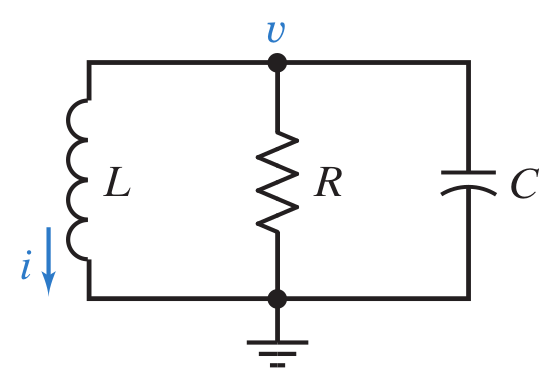
\includegraphics[height=2.5cm]{figure9.png}	
		\end{center}	
		\scalebox{0.8}{Answer: $v_n=-14e^{-t}+24e^{-2t}V$ }
		\end{column}
	\end{columns}
\end{tabular}
\end{frame}
% ----------------- NOVO SLIDE --------------------------------
\begin{frame}[fragile]
	\frametitle{Natural Response of an Overdamped Second-Order Circuit}
\begin{tabular}{ll}
	\begin{columns}
		\begin{column}{1\textwidth}  %%<--- here
		\textbf{EXERCISE 9.4-2} - Find the natural response of RLC circuit Below when $R=6 \Omega$, $L=7H$, and $C=\frac{1}{42}F$.
		The initial conditions are $v(0)=0$ and $i(0)=10A$.\\
		\begin{center}
    			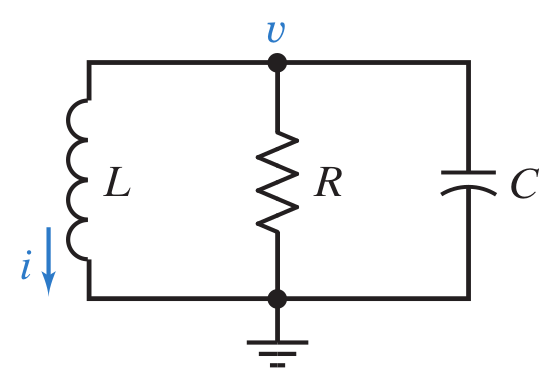
\includegraphics[height=2.5cm]{figure9.png}	
		\end{center}	
		\scalebox{0.8}{Answer: $v_n=-84(e^{-t}-e^{-6t})V$ }
		\end{column}
	\end{columns}
\end{tabular}
\end{frame}
% ----------------- NOVA SECÇÂO -----------------------------
\section{Natural Response of the Critically Damped Unforced Parallel RLC Circuit (9.5)}
% ----------------- NOVO SLIDE --------------------------------
\begin{frame}[fragile]
	\frametitle{Natural Response of the Critically Damped Unforced}
\begin{tabular}{ll}
	\begin{columns}
		\begin{column}{1\textwidth}  %%<--- here
Again we consider the parallel RLC circuit, and here we will determine the special case when the
characteristic equation has two equal real roots. Two real, equal roots occur when $\alpha^2=\omega^2$. \newline
		\end{column}
	\end{columns}\\
	\begin{columns}
		\begin{column}{.5\textwidth}  %%<--- here
\small		Let us assume that $s_1=s_2$ and proceed to find $v_n(t)$. We write the natural response as the sum of two
exponentials as
\begin{eqnarray} v_n=A_1e^{s_1t}+A_2e^{s_2t}=A_3e^{s_1t} \end{eqnarray}
Because the two roots are equal, we have only one undetermined constant, but we
still have two initial conditions to satisfy. 
		\end{column}

		\begin{column}{.5\textwidth}  %%<--- here
		
\small		Clearly, Eq. (1) is not the total solution for the natural
response of a critically damped circuit. \newline \newline
		Thus, we need the solution that will contain two arbitrary constants, so
with some foreknowledge, we try the solution
\begin{center} $v_n=(A_1t+A_2)e^{s_1t}$ \end{center}
		\end{column}
	\end{columns}
	
\end{tabular}	
\end{frame}
% ----------------- NOVO SLIDE --------------------------------
\begin{frame}[fragile]
	\frametitle{Natural Response of the Critically Damped Unforced}
\begin{tabular}{ll}
	\begin{columns}
		\begin{column}{1\textwidth}  %%<--- here
		\textbf{EXERCISE 9.5-1} - A parallel RLC circuit has $R=10 \Omega$, $C = 1 mF$, $L = 0.4 H$, $v(0) = 8 V$, and
$i(0) = 0$. Find the natural response $v_n (t)$ for $t < 0$.
		\begin{center}
    			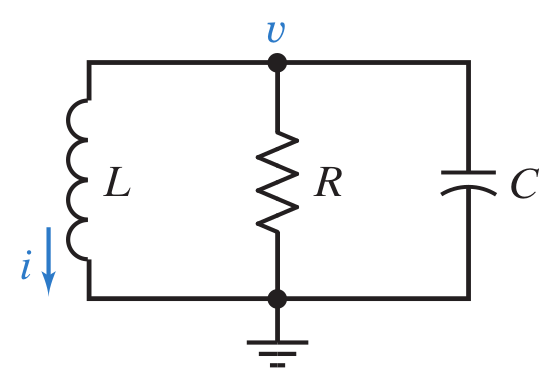
\includegraphics[height=2.5cm]{figure9.png}	
		\end{center}	
		\scalebox{0.8}{Answer: $v_n(t)=(8-400t)e^{-50t}V$ }
		\end{column}
	\end{columns}
\end{tabular}
\end{frame}



% ----------------- NOVA SECÇÂO -----------------------------
\section{Natural Response of an Underdamped Unforced Parallel RLC Circuit (9.6)}
% ----------------- NOVO SLIDE --------------------------------
\begin{frame}[fragile]
	\frametitle{Natural Response of an Underdamped Unforced}
\begin{tabular}{ll}
	\begin{columns}
		\begin{column}{1\textwidth}  %%<--- here
The characteristic equation of the parallel RLC circuit will have two complex conjugate roots when
$\alpha^2< \omega^2_0$ . \newline
		\end{column}
	\end{columns}\\
	\begin{columns}
		\begin{column}{.5\textwidth}  %%<--- here
		This condition is met when
		
		\begin{center}
		$LC<(2RC)^2$ \\
	%	 $s_{1,2}=-\alpha \pm \sqrt{\alpha^2-\omega_0^2}$, \ $\omega_d=\sqrt{\omega_0^2-\alpha^2}$ \ and \ $s_{1,2}=-\alpha \pm j\omega_d$
		  $s_{1,2}=-\alpha \pm \sqrt{\alpha^2-\omega_0^2}$\\
		  $s_{1,2}=-\alpha \pm j\sqrt{\omega_0^2-\alpha^2}$\\
		\end{center}
The complex roots lead to an oscillatory-type response.
		

		
		
		\end{column}

		\begin{column}{.5\textwidth}  %%<--- here
		
\small		We define the square root $\sqrt{\omega_0^2-\alpha^2}$ as
$\omega_d$, which we will call the damped resonant frequency. The factor $\alpha$, called the damping coefficient,
determines how quickly the oscillations subside. Then the roots are
\begin{center}
  $s_{1,2}=-\alpha \pm j\omega_d$\\
  $v_n=A_1e^{(-\alpha + j\omega_d)t}+A_2e^{(-\alpha - j\omega_d)t}$\\
  $v_n=e^{-\alpha t}(A_1e^{j\omega_d t}+A_2e^{- j\omega_d t})$\\
  $v_n=e^{-\alpha t}(B_1 \cos{\omega_d}+B_2 \sin {\omega_d t})$\\
\end{center}



		\end{column}
	\end{columns}
	
\end{tabular}	
\end{frame}

% ----------------- NOVO SLIDE --------------------------------
\begin{frame}[fragile]
	\frametitle{Natural Response of an Underdamped Unforced}
\begin{tabular}{ll}
	\begin{columns}
		\begin{column}{1\textwidth}  %%<--- here
		\textbf{EXERCISE 9.6-1} - Consider the parallel RLC circuit when $R=25/3 \Omega$, $L = 0.1 H$, $C = 1 mF$, $v(0) = 10 V$, and $i(0) = 0.6 A$. Find the
natural response $v_n (t)$ for $t > 0$.
		
		
		\begin{center}
    			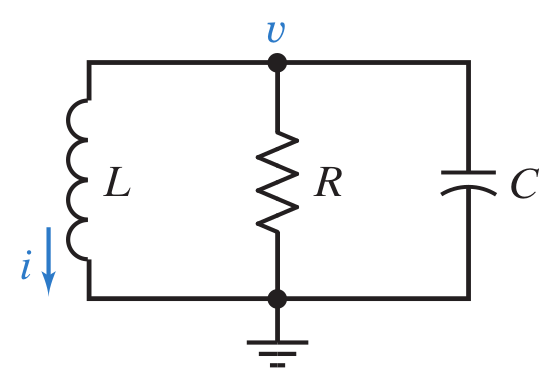
\includegraphics[height=2.5cm]{figure9.png}	
		\end{center}	
		\scalebox{0.8}{Answer: $v_n(t)=10e^{-60t} \cos{(80 t)} \ V$ }
		\end{column}
	\end{columns}
\end{tabular}
\end{frame}




% ----------------- NOVA SECÇÂO -----------------------------
\section{Forced Response of an RLC Circuit (9.7)}
% ----------------- NOVO SLIDE --------------------------------
\begin{frame}[fragile]
	\frametitle{Forced Response}

    		\begin{tabular}{ll}		
    		\begin{columns}
		\begin{column}{1\textwidth}  %%<--- here
 		The response to a forcing
function will often be of the same form as the forcing function.
		\end{column}
	        \end{columns}\\	
	\begin{columns}
	  \begin{column}{.5\textwidth}  %%<--- here
\begin{center}
\small	 \begin{tabular}{ |c|c| } 
\hline

 \multicolumn{2}{|c|}{\textbf{Forced Responses}} \\

 \hline

 Forcing Function & Assumed Response  \\ 
 $K$ & $A$  \\ 
 $Kt$ & $At+B$  \\
 $Kt^2$ & $At^2+Bt+C$  \\ 
 $K \sin{\omega t}$ & $A \sin{\omega t} + B \cos{\omega t}$  \\ 
 $Ke^{at}$ & $Ae^{-at}$ or $Ate^{-at}$  \\ 
 \hline
\end{tabular}
\end{center}
	  \end{column}
  \begin{column}{.5\textwidth}  %%<--- here
  Again, we consider the differential equation for the second-order circuit as \\
 \begin{center} $\frac{d^2x}{dt^2}+a_1\frac{dx}{dt}+a_0x=f(t)$ \end{center}
  Therefore, substituting $x_f$, we have
\small  \begin{eqnarray} \frac{d^2x_f}{dt^2}+a_1\frac{dx_f}{dt}+a_0x_f=f(t) \end{eqnarray}
		
We need to determine $x_f$ so that $x_f$ and its first and second derivatives all satisfy Eq. 2.

	  \end{column}
	\end{columns}
\end{tabular}	

\end{frame}
% ----------------- NOVO SLIDE --------------------------------
\begin{frame}[fragile]
	\frametitle{Forced Response to an Exponential Input}
\begin{tabular}{ll}
	\begin{columns}
		\begin{column}{1\textwidth}  %%<--- here
		\textbf{EXERCISE 9.7-1} - Find the forced response for the inductor current $i_f$ for the parallel RLC
circuit shown in Figure Below when $i_s = 8e^{-2t} A$. Let $R = 6 \Omega$, $L = 7 H$, and
$C = 1/42 F$.
		
		
		\begin{center}
    			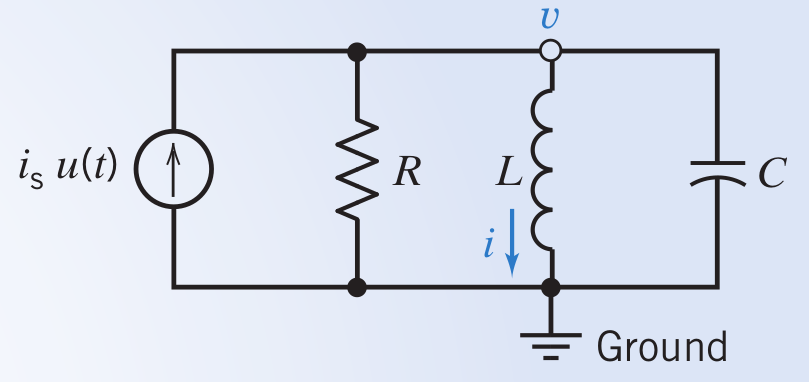
\includegraphics[height=2.5cm]{figure10.png}	
		\end{center}	
		\scalebox{0.8}{Answer: $i_f(t)=-12e^{-2t} \ A$ }
		\end{column}
	\end{columns}
\end{tabular}
\end{frame}
% ----------------- NOVA SECÇÂO -----------------------------
\section{Complete Response of an RLC Circuit (9.8)}
% ----------------- NOVO SLIDE --------------------------------
\begin{frame}[fragile]
	\frametitle{Complete Response of a Second-Order Circuit}

    		\begin{tabular}{ll}		
    		\begin{columns}
		\begin{column}{1\textwidth}  %%<--- here
 The \textbf{complete response} is the sum of the natural response and the forced response; thus,
\begin{center} $x= x_n + x_f$ \end{center}
		\end{column}
	        \end{columns}\\	
	\begin{columns}
	  \begin{column}{.5\textwidth}  %%<--- here
	\textbf{EXERCISE 9.8-1} - 
	Find the complete response $v(t)$ for $t > 0$ for the circuit of
Figure. Assume the circuit is at steady state at $t = 0$.

	  \end{column}
	  \begin{column}{.5\textwidth}  %%<--- here
	\begin{center}
    			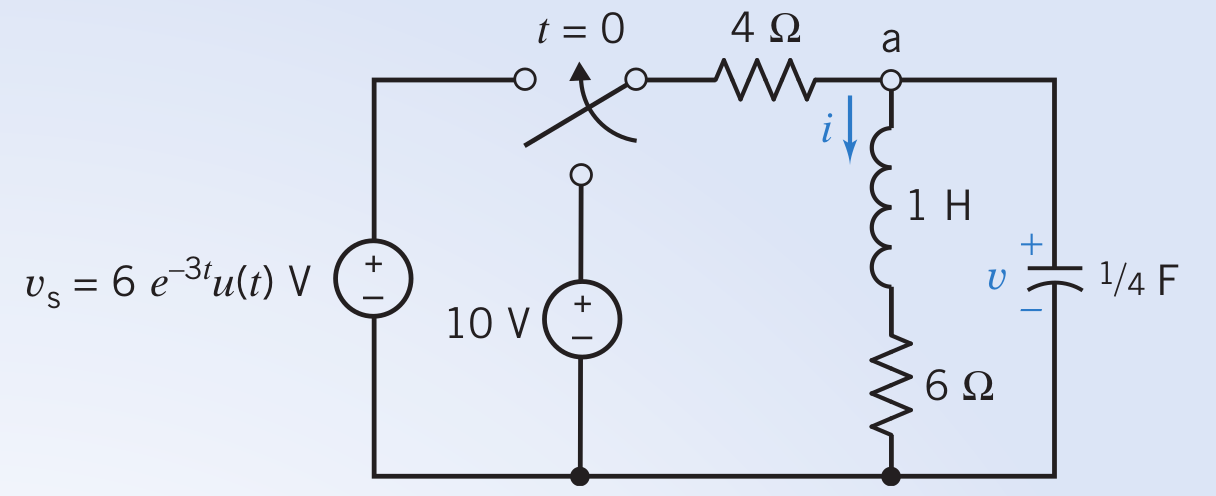
\includegraphics[height=3cm]{figure11.png}	
		\end{center}	
	  \end{column}
	\end{columns}
\end{tabular}	

\end{frame}

\end{document} 

